\documentclass[tikz,border=0pt]{standalone}
\usepackage[T1]{fontenc}
\usepackage[scaled=0.94]{helvet}
\renewcommand{\familydefault}{\sfdefault}
\usepackage{amsmath}
\DeclareMathSizes{7}{7}{7}{7}
\hyphenpenalty=10000
\exhyphenpenalty=10000
\usepackage{xcolor}
\usetikzlibrary{arrows.meta,calc,patterns,positioning,fit}

\pgfdeclarelayer{background}
\pgfsetlayers{background,main}

\definecolor{OIblue}{HTML}{0072B2}
\definecolor{OIorange}{HTML}{E69F00}
\definecolor{OIgreen}{HTML}{009E73}
\definecolor{OIred}{HTML}{D55E00}
\definecolor{OIpurple}{HTML}{CC79A7}
\definecolor{OIsky}{HTML}{56B4E9}
\definecolor{OIdark}{HTML}{343A40}

\newcommand{\paneltitle}[1]{{\sffamily\bfseries\fontsize{9}{10.5}\selectfont #1}}
\newcommand{\boxtitle}[1]{{\sffamily\bfseries\fontsize{8}{9.5}\selectfont #1}}
\newcommand{\bodyfont}[1]{{\sffamily\fontsize{7}{7.5}\selectfont #1}}

\tikzset{
  every node/.style={font=\sffamily\fontsize{7}{7.5}\selectfont},
  panel/.style={draw=gray!55,fill=gray!2,rounded corners=2pt,line width=.55pt,inner sep=2mm},
  sourcebox/.style={draw=gray!55,fill=white,rounded corners=1.2pt,line width=.45pt,
                    text width=3.72cm,align=center,inner sep=1mm},
  methodbox/.style={draw=gray!60,fill=white,rounded corners=1.3pt,line width=.5pt,
                    align=center,inner sep=1.5mm},
  flow/.style={-{Latex[length=1mm,width=.8mm]},draw=OIdark!82,line width=.65pt},
  queryflow/.style={-{Latex[length=1mm,width=.8mm]},draw=OIpurple!90!black,line width=.7pt},
  teacherflow/.style={-{Latex[length=1mm,width=.8mm]},draw=OIdark!75,dashed,line width=.7pt},
  poscell/.style={draw=gray!55,fill=OIblue,line width=.35pt},
  negcell/.style={draw=gray!55,fill=white,line width=.35pt},
  unknowncell/.style={draw=gray!60,fill=gray!10,pattern=north east lines,pattern color=gray!65,line width=.35pt}
}

\newcommand{\cellpos}{\tikz[baseline=-.55ex]\node[poscell,minimum width=4.2mm,minimum height=2.5mm,inner sep=0pt,font=\sffamily\fontsize{7}{7}\selectfont,text=white]{1};}
\newcommand{\cellneg}{\tikz[baseline=-.55ex]\node[negcell,minimum width=4.2mm,minimum height=2.5mm,inner sep=0pt,font=\sffamily\fontsize{7}{7}\selectfont,text=gray!70]{0};}
\newcommand{\cellunk}{\tikz[baseline=-.55ex]\node[unknowncell,minimum width=4.2mm,minimum height=2.5mm,inner sep=0pt,font=\sffamily\fontsize{7}{7}\selectfont]{?};}
\newcommand{\stage}[1]{\tikz[baseline=-.55ex]\node[draw=gray!55,fill=OIblue!10,rounded corners=.5pt,minimum width=3.5mm,minimum height=4mm,inner sep=0pt,font=\sffamily\fontsize{7}{7}\selectfont]{#1};}
\newcommand{\tracegreen}{\tikz[baseline=-.55ex,x=.60mm,y=1mm]\draw[OIgreen!80!black,line width=.45pt] (0,1)--(2,1)--(3,1.4)--(4,.9)--(5,.2)--(6,2.5)--(7,.7)--(8,1)--(11,1)--(12,1.4)--(13,.9)--(14,.2)--(15,2.5)--(16,.7)--(17,1)--(20,1);}
\newcommand{\traceorange}{\tikz[baseline=-.55ex,x=.60mm,y=1mm]\draw[OIorange!90!black,line width=.45pt] (0,1)--(2,1)--(3,1.4)--(4,.9)--(5,.2)--(6,2.5)--(7,.7)--(8,1)--(11,1)--(12,1.4)--(13,.9)--(14,.2)--(15,2.5)--(16,.7)--(17,1)--(20,1);}
\newcommand{\tracepurple}{\tikz[baseline=-.55ex,x=.60mm,y=1mm]\draw[OIpurple!90!black,line width=.45pt] (0,1)--(2,1)--(3,1.4)--(4,.9)--(5,.2)--(6,2.5)--(7,.7)--(8,1)--(11,1)--(12,1.4)--(13,.9)--(14,.2)--(15,2.5)--(16,.7)--(17,1)--(20,1);}
\newcommand{\crossicon}{\tikz[baseline=-.55ex]\draw[OIred,line width=1pt] (0,0)--(2.6mm,2.6mm) (0,2.6mm)--(2.6mm,0);}

\begin{document}
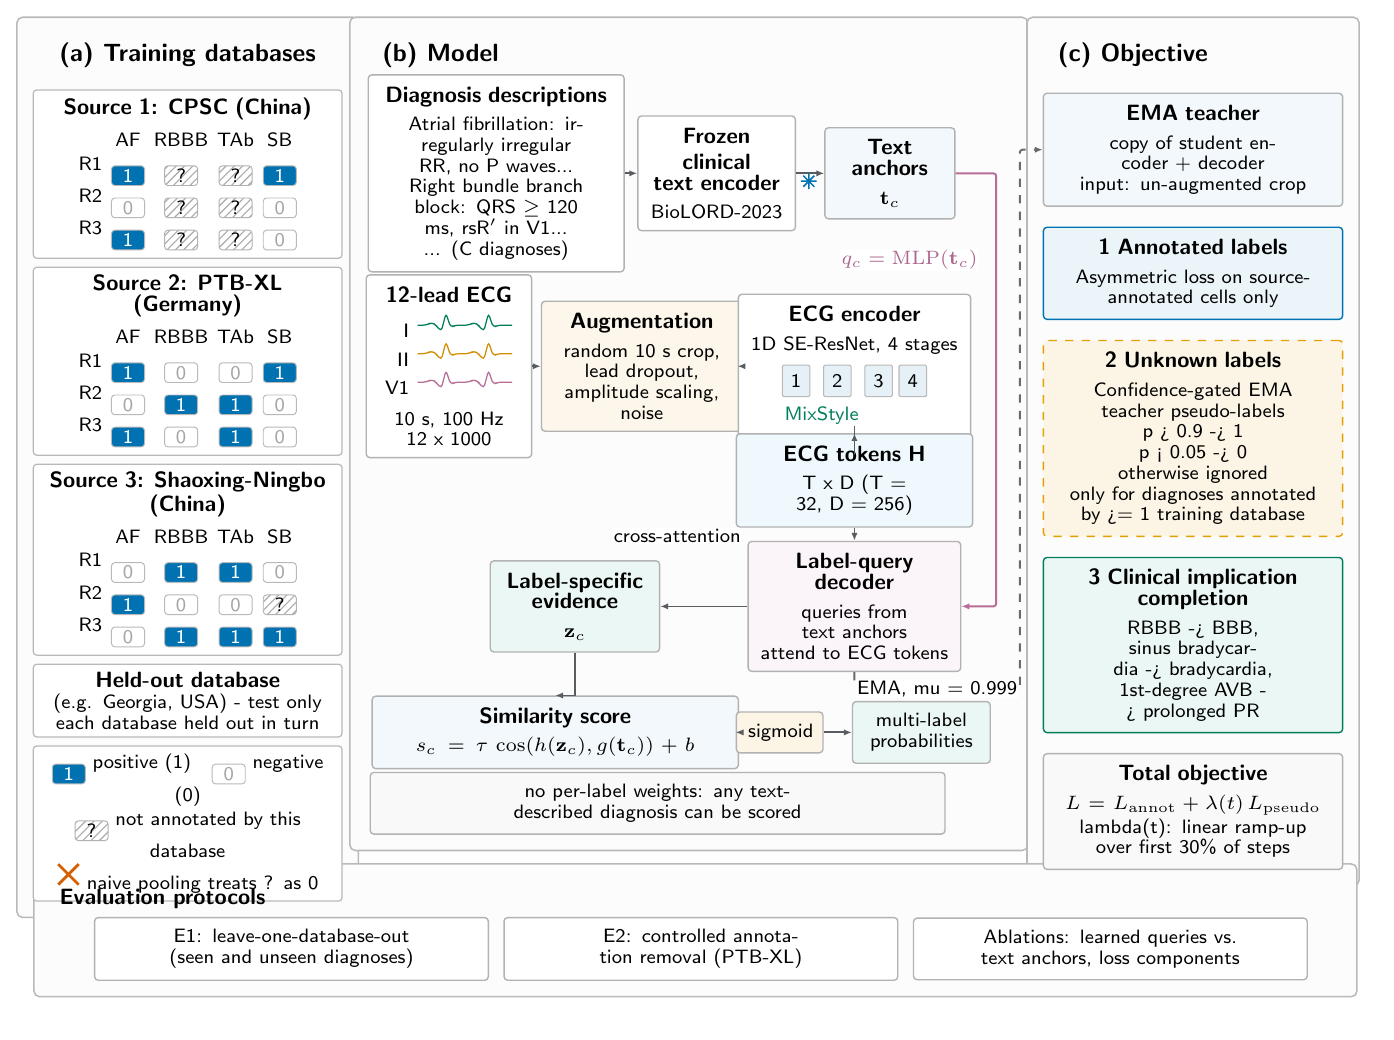
\begin{tikzpicture}[x=1cm,y=1cm,node distance=2mm]
  \path[use as bounding box] (0,0) rectangle (17,12.5);
  \begin{scope}[yshift=1cm]

  % Panel titles: 9 pt bold, inside the panel frames
  \node[anchor=west] (atitle) at (.28,11.15) {\paneltitle{(a) Training databases}};
  \node[anchor=west] (btitle) at (4.38,11.15) {\paneltitle{(b) Model}};
  \node[anchor=west] (ctitle) at (12.96,11.15) {\paneltitle{(c) Objective}};

  % Panel (a): source-specific illustrative annotation grids
  \node[sourcebox,below=1.5mm of atitle.south] (src1) {%
    \parbox{3.72cm}{\centering
      \boxtitle{Source 1: CPSC (China)}\\[1mm]
      {\sffamily\fontsize{7}{7.5}\selectfont
      \setlength{\tabcolsep}{1.6pt}\renewcommand{\arraystretch}{1.12}
      \begin{tabular}{@{}c cccc@{}}
        & AF & RBBB & TAb & SB\\
        R1 & \cellpos & \cellunk & \cellunk & \cellpos\\
        R2 & \cellneg & \cellunk & \cellunk & \cellneg\\
        R3 & \cellpos & \cellunk & \cellunk & \cellneg
      \end{tabular}}}};
  \node[sourcebox,below=1mm of src1.south] (src2) {%
    \parbox{3.72cm}{\centering
      \boxtitle{Source 2: PTB-XL (Germany)}\\[1mm]
      {\sffamily\fontsize{7}{7.5}\selectfont
      \setlength{\tabcolsep}{1.6pt}\renewcommand{\arraystretch}{1.12}
      \begin{tabular}{@{}c cccc@{}}
        & AF & RBBB & TAb & SB\\
        R1 & \cellpos & \cellneg & \cellneg & \cellpos\\
        R2 & \cellneg & \cellpos & \cellpos & \cellneg\\
        R3 & \cellpos & \cellneg & \cellpos & \cellneg
      \end{tabular}}}};
  \node[sourcebox,below=1mm of src2.south] (src3) {%
    \parbox{3.72cm}{\centering
      \boxtitle{Source 3: Shaoxing-Ningbo (China)}\\[1mm]
      {\sffamily\fontsize{7}{7.5}\selectfont
      \setlength{\tabcolsep}{1.6pt}\renewcommand{\arraystretch}{1.12}
      \begin{tabular}{@{}c cccc@{}}
        & AF & RBBB & TAb & SB\\
        R1 & \cellneg & \cellpos & \cellpos & \cellneg\\
        R2 & \cellpos & \cellneg & \cellneg & \cellunk\\
        R3 & \cellneg & \cellpos & \cellpos & \cellpos
      \end{tabular}}}};
  \node[sourcebox,below=1mm of src3.south] (heldout) {%
    \parbox{3.72cm}{\centering
      \boxtitle{Held-out database}\\
      \bodyfont{(e.g. Georgia, USA) - test only\\
      each database held out in turn}}};
  \node[sourcebox,below=1mm of heldout.south] (legend) {%
    \parbox{3.72cm}{\centering
      \bodyfont{\cellpos\ positive (1)\quad \cellneg\ negative (0)\\[1pt]
      \cellunk\ not annotated by this database\\[1pt]
      \crossicon\ naive pooling treats ? as 0}}};

  % Panel (b): diagnosis text, frozen encoder, and text anchors
  \node[methodbox,text width=2.95cm] (descriptions) at (5.95,9.65) {%
    \boxtitle{Diagnosis descriptions}\\[1mm]
    \bodyfont{Atrial fibrillation: irregularly irregular RR, no P waves...\\
    Right bundle branch block: QRS $\geq$ 120 ms, rsR$'$ in V1...\\
    ... (C diagnoses)}};
  \node[methodbox,text width=1.70cm] (textenc) at (8.75,9.65) {%
    \boxtitle{Frozen clinical\\text encoder}\\[1mm]
    \bodyfont{BioLORD-2023}};
  \node[methodbox,text width=1.35cm,fill=OIblue!5] (anchors) at (10.95,9.65) {%
    \boxtitle{Text anchors}\\[1mm]
    \bodyfont{$\mathbf{t}_c$}};
  \draw[flow] (descriptions.east)--(textenc.west);
  \draw[flow] (textenc.east)--(anchors.west);

  % Snowflake icon beside the frozen text encoder
  \draw[OIblue,line width=.55pt]
    (9.82,9.55)--(10.02,9.55)
    (9.92,9.45)--(9.92,9.65)
    (9.85,9.48)--(9.99,9.62)
    (9.85,9.62)--(9.99,9.48);

  % Panel (b): 12-lead ECG, augmentation, and encoder
  \node[methodbox,text width=1.80cm] (ecg) at (5.35,7.20) {%
    \boxtitle{12-lead ECG}\\[1mm]
    {\sffamily\fontsize{7}{7.5}\selectfont
    \begin{tabular}{@{}r@{\hspace{1mm}}l@{}}
      I & \tracegreen\\[-1pt]
      II & \traceorange\\[-1pt]
      V1 & \tracepurple
    \end{tabular}}\\[1mm]
    \bodyfont{10 s, 100 Hz\\12 x 1000}};
  \node[methodbox,text width=2.25cm,fill=OIorange!8] (augment) at (7.80,7.20) {%
    \boxtitle{Augmentation}\\[1mm]
    \bodyfont{random 10 s crop,\\
    lead dropout,\\
    amplitude scaling,\\
    noise}};
  \node[methodbox,text width=2.65cm] (encoder) at (10.50,7.20) {%
    \boxtitle{ECG encoder}\\[1mm]
    \bodyfont{1D SE-ResNet, 4 stages}\\[1mm]
    \setlength{\tabcolsep}{1pt}
    \begin{tabular}{@{}cccc@{}}
      \stage{1} & \stage{2} & \stage{3} & \stage{4}\\[5pt]
      \multicolumn{2}{c}{\bodyfont{\color{OIgreen!80!black}MixStyle}} &
      \multicolumn{2}{c}{}
    \end{tabular}};
  \draw[flow] (ecg.east)--(augment.west);
  \draw[flow] (augment.east)--(encoder.west);

  % ECG token representation below the encoder; decoder sits at least 3 mm below
  \node[methodbox,text width=2.70cm,fill=OIsky!10] (tokens) at (10.50,5.75) {%
    \boxtitle{ECG tokens H}\\[1mm]
    \bodyfont{T x D (T = 32, D = 256)}};
  \draw[flow] (encoder.south)--++(0,-2mm)|-(tokens.north);

  \node[methodbox,text width=2.40cm,fill=OIpurple!8] (decoder) at (10.50,4.15) {%
    \boxtitle{Label-query decoder}\\[1mm]
    \bodyfont{queries from text anchors\\
    attend to ECG tokens}};
  \node[methodbox,text width=1.85cm,fill=OIgreen!8] (evidence) at (6.95,4.15) {%
    \boxtitle{Label-specific\\evidence}\\[1mm]
    \bodyfont{$\mathbf{z}_c$}};
  \draw[flow] (decoder.west)--(evidence.east);
  \draw[flow] (tokens.south)--(decoder.north);
  \node[font=\sffamily\fontsize{7}{7.5}\selectfont,fill=white,inner sep=.5pt]
    at (8.25,5.05) {cross-attention};

  % Text-anchor query route along the right edge, clear of ECG tokens
  \draw[queryflow,rounded corners=1pt]
    (anchors.east)--(12.30,9.65)--(12.30,4.15)--(decoder.east);
  \node[font=\sffamily\fontsize{7}{7.5}\selectfont,text=OIpurple!85!black,fill=white,inner sep=.5pt]
    at (11.20,8.55) {$q_c=\mathrm{MLP}(\mathbf{t}_c)$};

  % Similarity score, sigmoid, probabilities, and open-vocabulary note
  \node[methodbox,text width=4.35cm,fill=OIblue!5] (score) at (6.70,2.55) {%
    \boxtitle{Similarity score}\\[1mm]
    \bodyfont{$s_c=\tau\,\cos\!\left(h(\mathbf{z}_c),g(\mathbf{t}_c)\right)+b$}};
  \node[methodbox,text width=.80cm,fill=OIorange!10] (sigmoid) at (9.55,2.55) {\bodyfont{sigmoid}};
  \node[methodbox,text width=1.45cm,fill=OIgreen!8] (prob) at (11.35,2.55) {%
    \bodyfont{multi-label\\probabilities}};
  \draw[flow] (score.east)--(sigmoid.west);
  \draw[flow] (sigmoid.east)--(prob.west);
  \draw[flow] (evidence.south) |-(score.north);
  \node[methodbox,text width=7.00cm,fill=gray!5] (openvocab) at (8.00,1.65) {%
    \bodyfont{no per-label weights: any text-described diagnosis can be scored}};

  % Panel (c): EMA teacher and stacked annotation-aware objectives
  \node[methodbox,text width=3.50cm,fill=OIblue!5] (teacher) at (14.80,9.95) {%
    \boxtitle{EMA teacher}\\[1mm]
    \bodyfont{copy of student encoder + decoder\\
    input: un-augmented crop}};
  \node[methodbox,text width=3.50cm,fill=OIblue!8,draw=OIblue,below=2.5mm of teacher] (annot) {%
    \boxtitle{1  Annotated labels}\\[1mm]
    \bodyfont{Asymmetric loss on source-annotated cells only}};
  \node[methodbox,text width=3.50cm,fill=OIorange!10,draw=OIorange,dashed,below=2.5mm of annot] (pseudo) {%
    \boxtitle{2  Unknown labels}\\[1mm]
    \bodyfont{Confidence-gated EMA teacher pseudo-labels\\
    p > 0.9 -> 1\\
    p < 0.05 -> 0\\
    otherwise ignored\\
    only for diagnoses annotated by >= 1 training database}};
  \node[methodbox,text width=3.50cm,fill=OIgreen!8,draw=OIgreen!80!black,below=2.5mm of pseudo] (clinical) {%
    \boxtitle{3  Clinical implication}\\\boxtitle{completion}\\[1mm]
    \bodyfont{RBBB -> BBB,\\
    sinus bradycardia -> bradycardia,\\
    1st-degree AVB -> prolonged PR}};
  \node[methodbox,text width=3.50cm,fill=gray!5,below=2.5mm of clinical] (objective) {%
    \boxtitle{Total objective}\\[1mm]
    \bodyfont{$\displaystyle L = L_{\mathrm{annot}} + \lambda(t)\, L_{\mathrm{pseudo}}$}\\[1pt]
    \bodyfont{lambda(t): linear ramp-up over first 30\% of steps}};

  % EMA student-to-teacher path uses the outer right lane, away from the query arrow
  \draw[teacherflow,rounded corners=1pt]
    (decoder.south)--++(0,-2mm)--(12.60,3.10)--(12.60,9.95)--(teacher.west);
  \node[font=\sffamily\fontsize{7}{7.5}\selectfont,fill=white,inner sep=.5pt]
    at (11.55,3.10) {EMA, mu = 0.999};

  \end{scope}

  % Bottom evaluation protocol strip
  \node[anchor=west] (evaltitle) at (.28,1.43) {\boxtitle{Evaluation protocols}};
  \node[methodbox,text width=4.70cm] (eval1) at (3.35,.80) {%
    \bodyfont{E1: leave-one-database-out\\(seen and unseen diagnoses)}};
  \node[methodbox,text width=4.70cm] (eval2) at (8.55,.80) {%
    \bodyfont{E2: controlled annotation removal (PTB-XL)}};
  \node[methodbox,text width=4.70cm] (eval3) at (13.75,.80) {%
    \bodyfont{Ablations: learned queries vs. text anchors, loss components}};

  % Panel frames are fitted around the content on the background layer
  \begin{pgfonlayer}{background}
    \begin{scope}[yshift=1cm]
      \coordinate (aNW) at (.32,11.18); \coordinate (aSE) at (3.92,1.75);
      \coordinate (bNW) at (4.42,11.18); \coordinate (bSE) at (12.50,1.25);
      \coordinate (cNW) at (13.00,11.18); \coordinate (cSE) at (16.68,1.75);
      \node[panel,fit=(aNW)(aSE)(atitle)(src1)(src2)(src3)(heldout)(legend)] {};
      \node[panel,fit=(bNW)(bSE)(btitle)(descriptions)(textenc)(anchors)(ecg)(augment)(encoder)(tokens)(decoder)(evidence)(score)(sigmoid)(prob)(openvocab)] {};
      \node[panel,fit=(cNW)(cSE)(ctitle)(teacher)(annot)(pseudo)(clinical)(objective)] {};
    \end{scope}
    \coordinate (eNW) at (.32,1.57); \coordinate (eSE) at (16.68,.47);
    \node[panel,fit=(eNW)(eSE)(evaltitle)(eval1)(eval2)(eval3)] {};
  \end{pgfonlayer}
\end{tikzpicture}
\end{document}
